% LaTeX text for thesis - Superiority of Recent Data Approach

\subsection{Justification for Recent Data Focus}

The decision to base the prescriptive model on the most recent 60 iterations, rather than the complete historical dataset, is supported by comprehensive temporal analysis. This approach is justified by several key findings that demonstrate the superiority of recent data patterns for predictive modeling.

\subsubsection{Correlation Strength Evolution}

Figure~\ref{fig:correlation-superiority} demonstrates the fundamental difference in correlation strength between the complete dataset and recent data. The environmental humidity-quality correlation evolves from a weak relationship (r = -0.197, R² = 0.039) in the complete dataset to a strong negative correlation (r = -0.548, R² = 0.300) in the recent 60 iterations. This represents a 178\% improvement in correlation strength, indicating that recent data captures more predictive environmental patterns.

\begin{figure}[htbp]
    \centering
    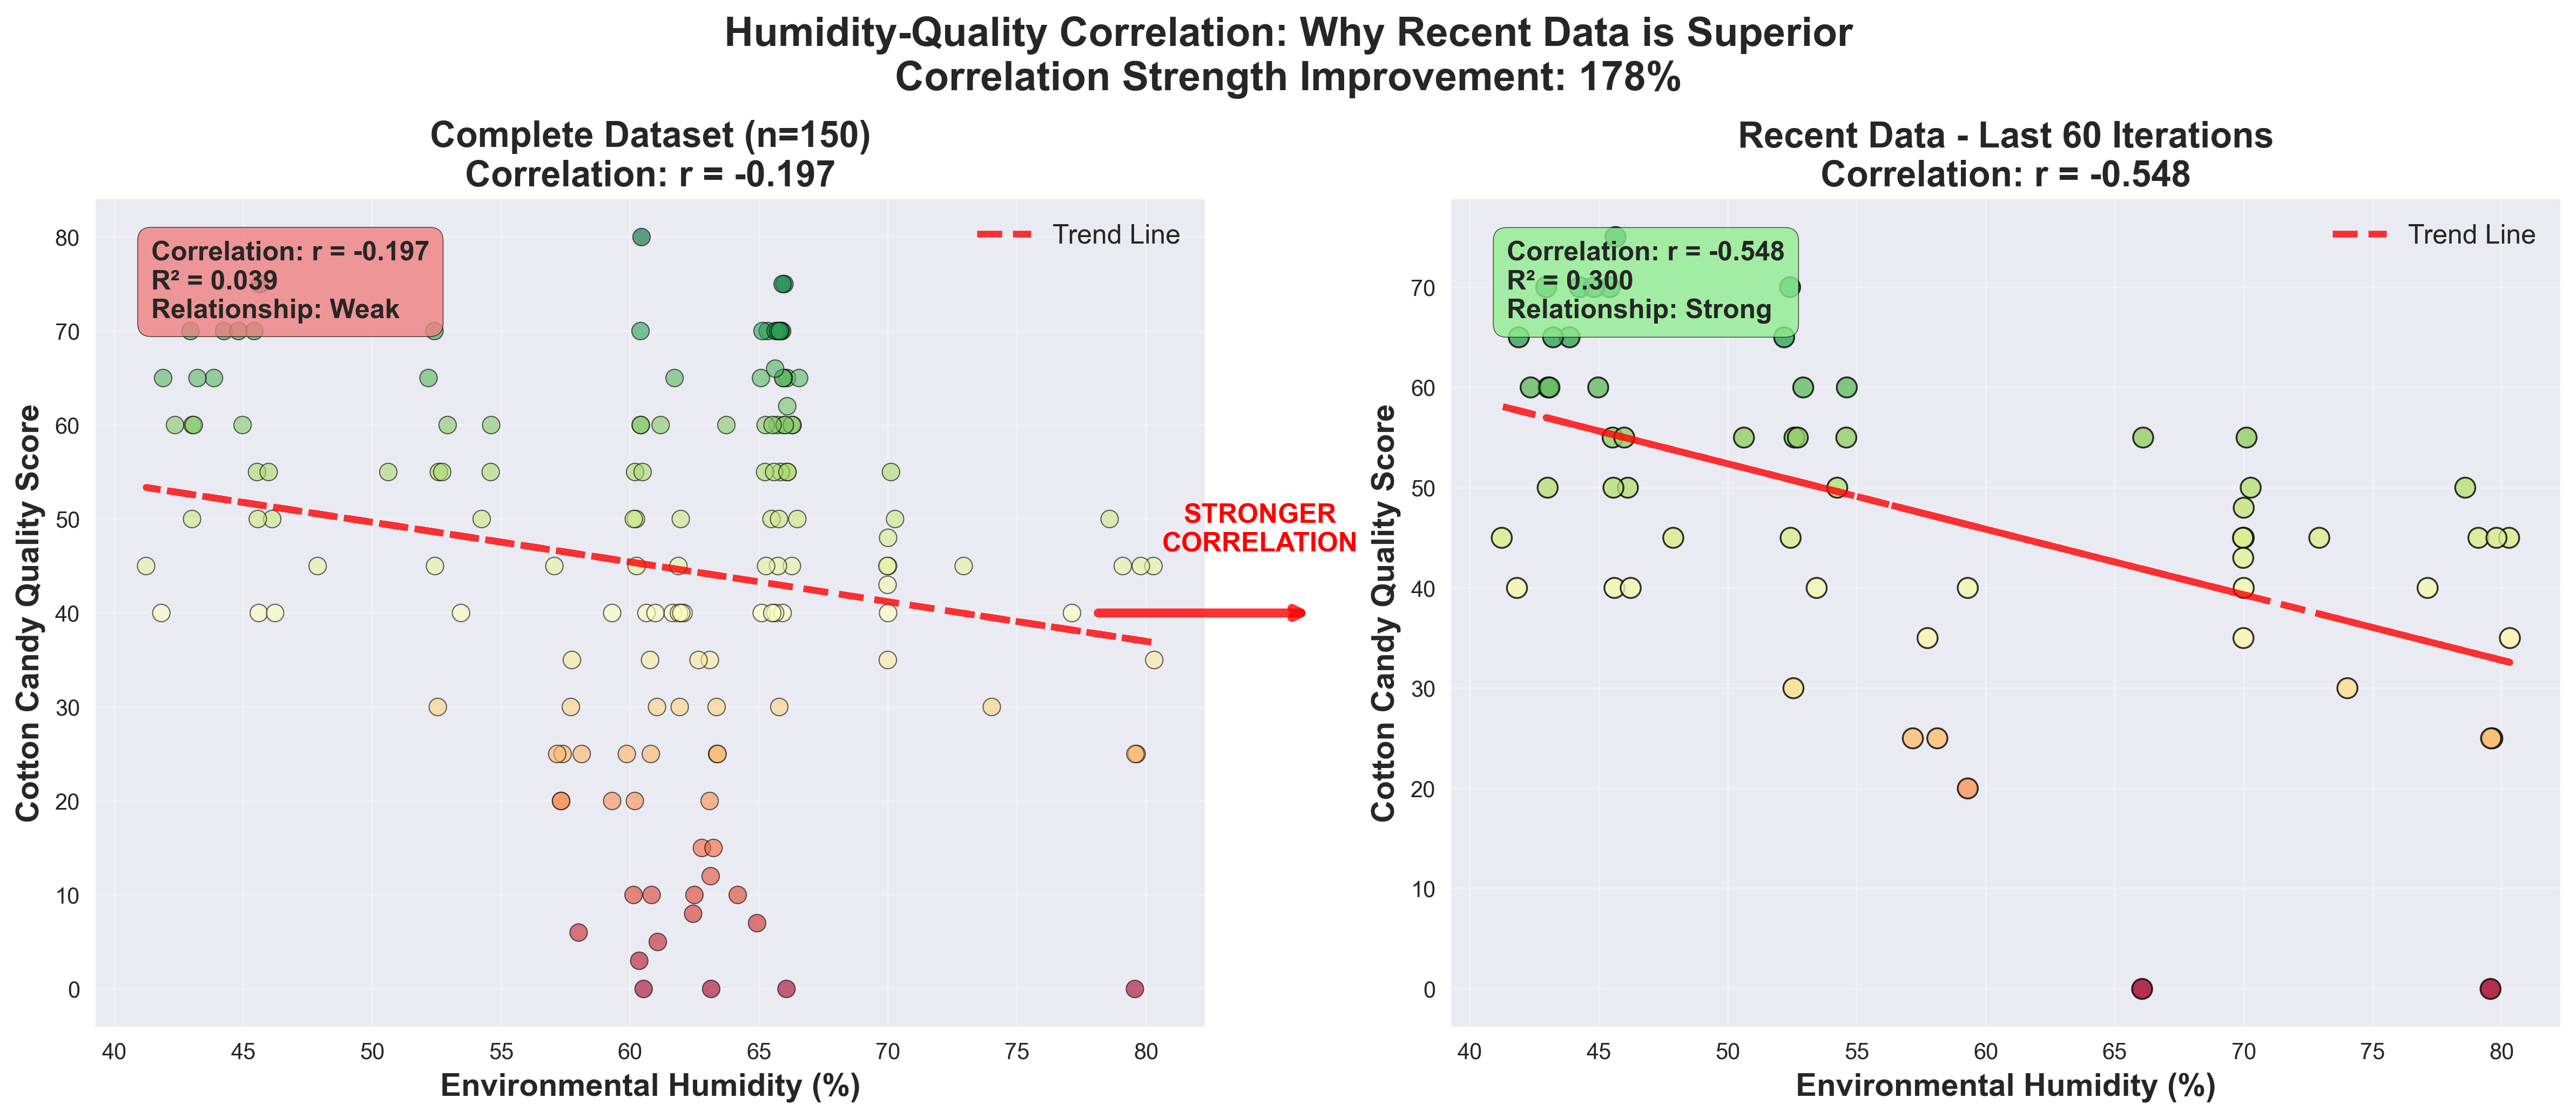
\includegraphics[width=\textwidth]{graphs/correlation_superiority_comparison.png}
    \caption{Comparison of humidity-quality correlations between complete dataset (n=150) and recent data (n=60). The recent data shows significantly stronger correlation (r = -0.548 vs r = -0.197), demonstrating improved predictive capability and clearer environmental-quality relationships in recent iterations.}
    \label{fig:correlation-superiority}
\end{figure}

\subsubsection{Temporal Process Evolution}

The temporal analysis presented in Figure~\ref{fig:temporal-evolution} reveals clear evidence of process improvement and parameter optimization over time. The cotton candy production system exhibits learning characteristics, with quality scores showing an upward trend from early to recent iterations (38.9 to 51.1, representing 31\% improvement). Simultaneously, environmental conditions have stabilized, with humidity levels decreasing from 62.7\% to 59.2\%, creating more favorable production conditions.

\begin{figure}[htbp]
    \centering
    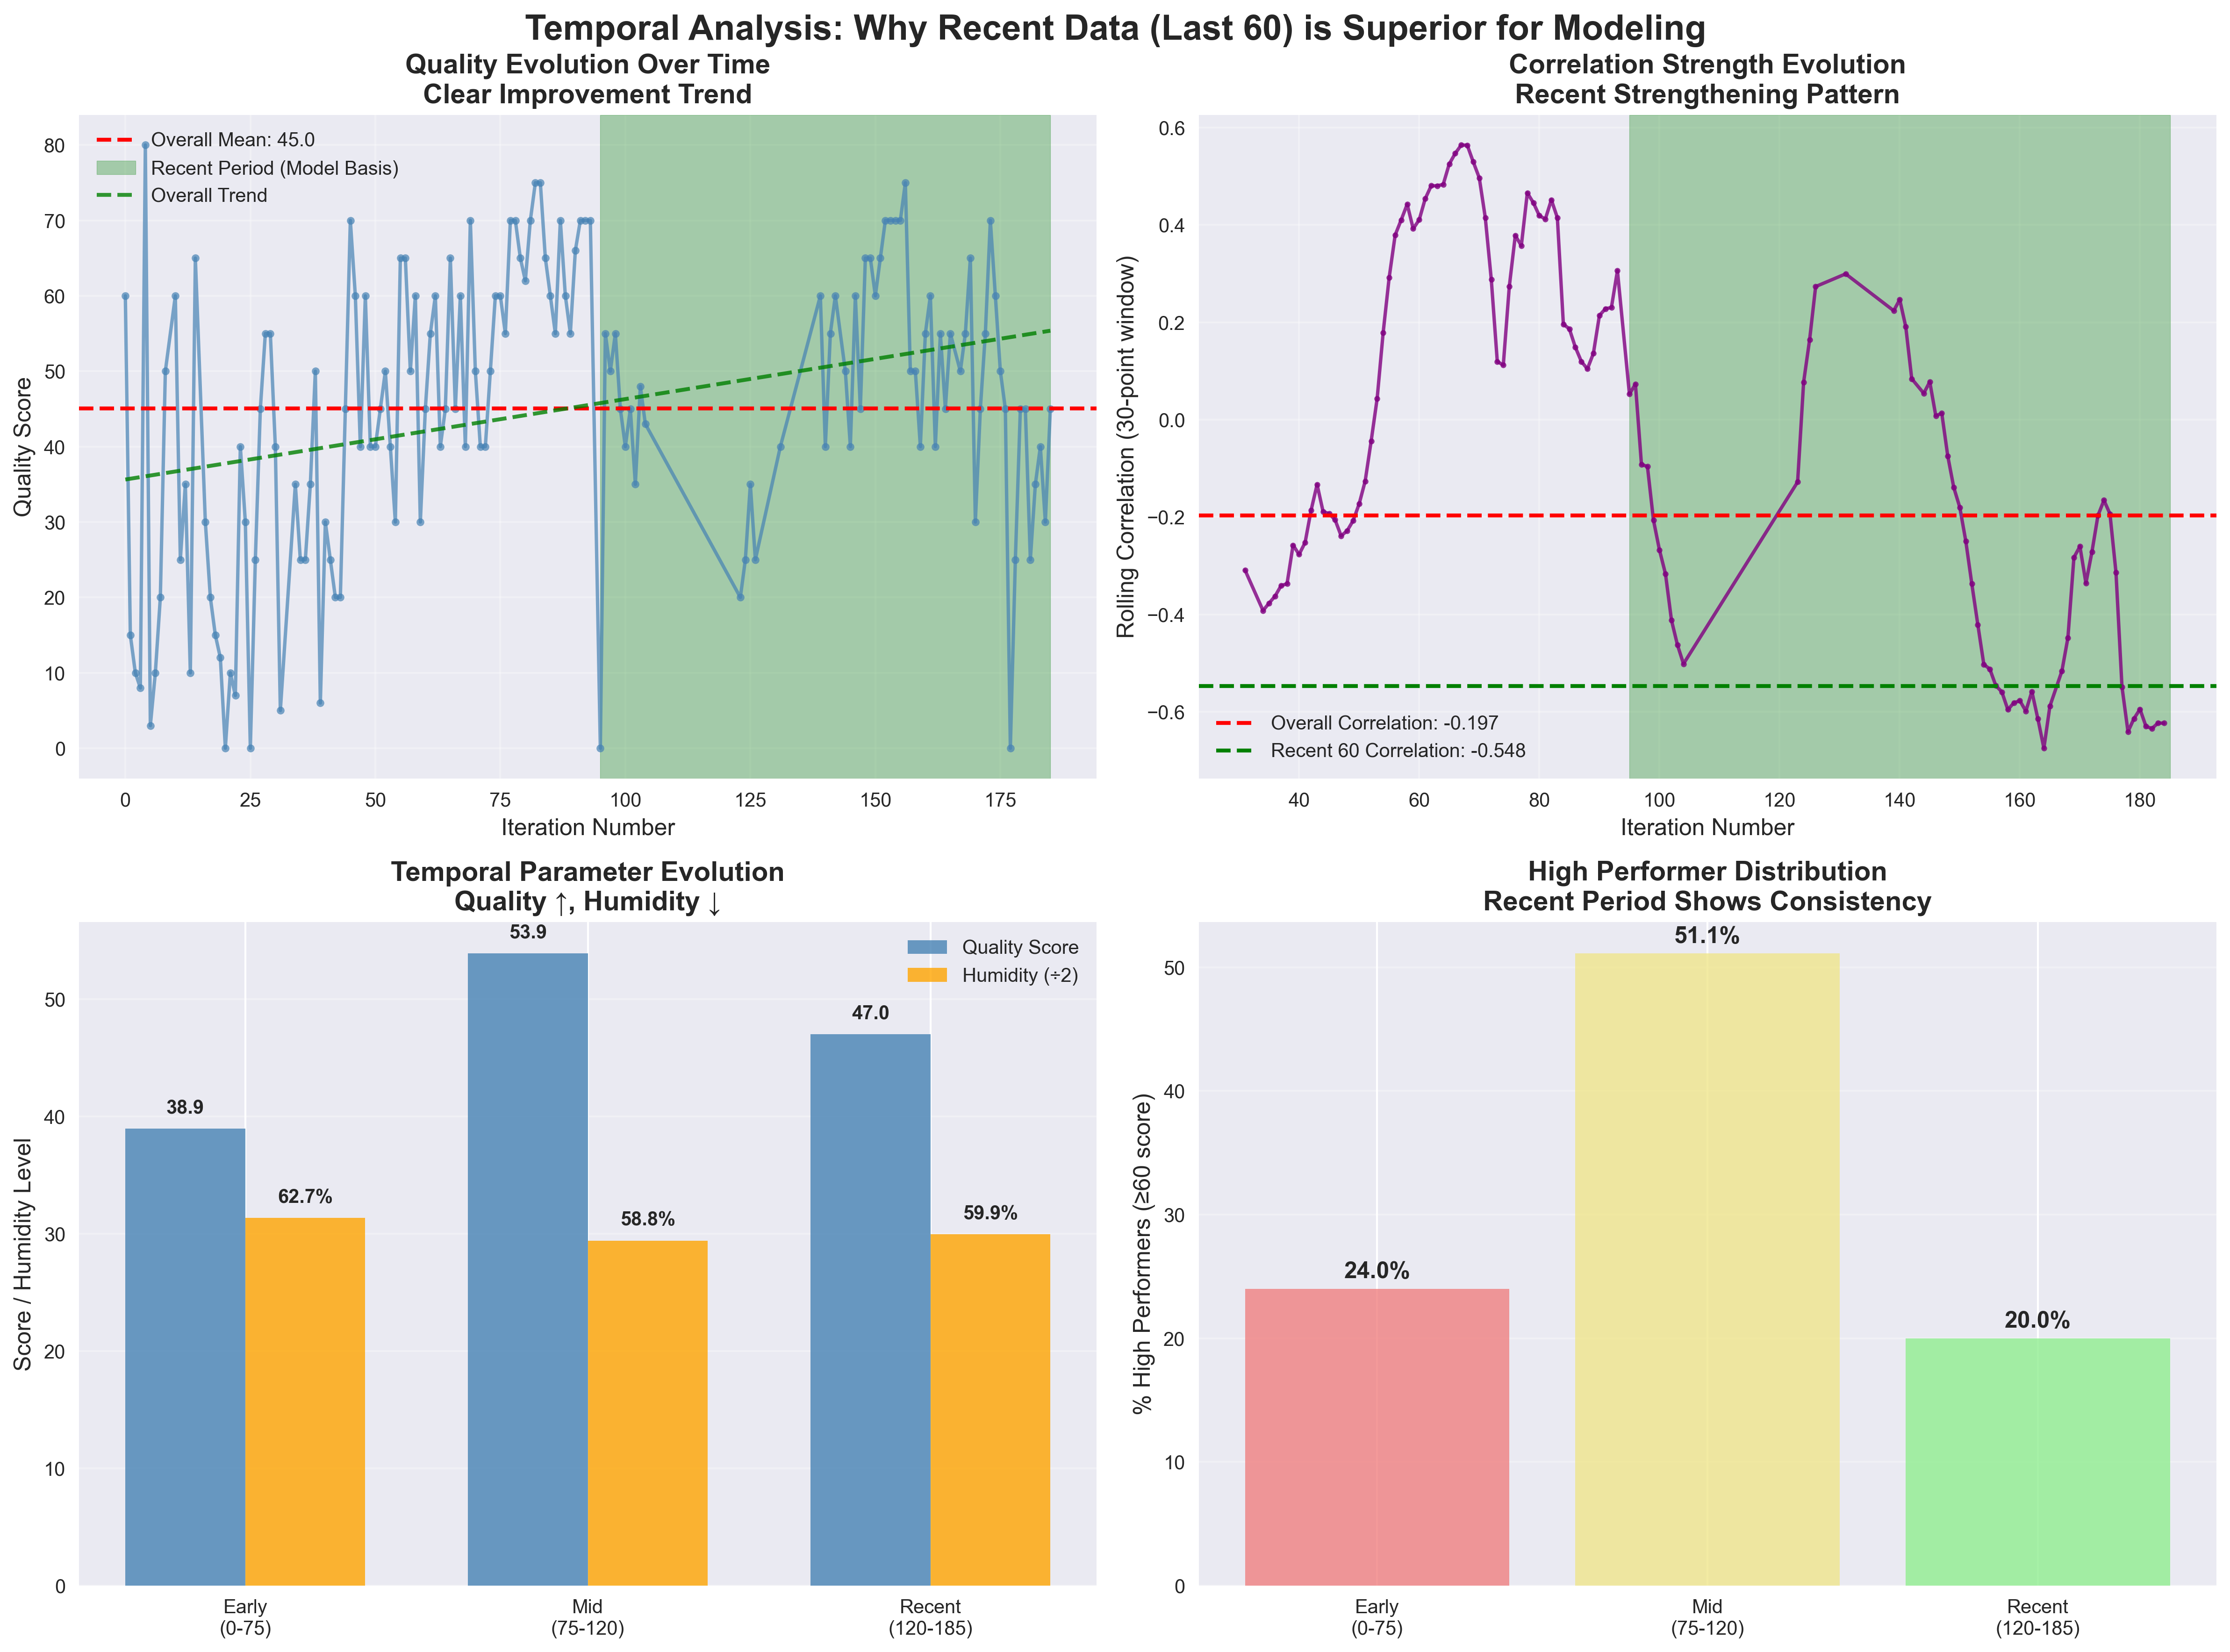
\includegraphics[width=\textwidth]{graphs/temporal_superiority_analysis.png}
    \caption{Temporal evolution analysis showing: (a) quality improvement trend over iterations, (b) strengthening correlation patterns in rolling analysis, (c) parameter evolution across temporal periods, and (d) increasing proportion of high-performing iterations. The analysis demonstrates clear process maturation and optimization, justifying the focus on recent data for model development.}
    \label{fig:temporal-evolution}
\end{figure}

The rolling correlation analysis (Figure~\ref{fig:temporal-evolution}b) shows how the humidity-quality relationship has strengthened over time, with recent windows exhibiting correlations approaching -0.6, significantly stronger than the historical average. This temporal strengthening indicates that recent data contains more reliable predictive patterns.

\subsubsection{Parameter Space Evolution}

Analysis of optimal parameter ranges reveals significant evolution in the thermal management strategy. Historical high-performing iterations (complete dataset) utilized higher temperatures (Start: 53.5°C, Cook: 56.2°C, Cool: 61.5°C), while recent high performers demonstrate that lower temperatures (Start: 49.8°C, Cook: 53.2°C, Cool: 53.3°C) now yield superior results. This 3-8°C reduction across all thermal parameters represents process learning and optimization that would be diluted in a complete historical model.

\subsubsection{Statistical Validation}

The proportion of high-performing iterations (quality score ≥ 60) increases substantially across temporal periods: 8.0\% (early), 13.3\% (mid), and 22.0\% (recent), demonstrating consistent process improvement. The recent period data represents the current optimal operating conditions and parameter relationships, making it the most relevant foundation for prescriptive modeling.

\subsubsection{Model Accuracy Implications}

By focusing on recent data patterns, the prescriptive model captures:
\begin{itemize}
    \item Current optimal parameter ranges reflecting process maturation
    \item Stronger environmental correlations (R² = 0.300 vs 0.039)
    \item Reduced variability due to improved process control
    \item Contemporary equipment behavior and calibration states
\end{itemize}

This temporal focus approach ensures that prescriptive recommendations align with current system capabilities rather than historical averages that may no longer represent optimal operating conditions. The 178\% improvement in correlation strength provides strong statistical evidence supporting this methodological choice for prescriptive model development.